\documentclass{replab}
\usepackage{lipsum}

% --- Información del documento ---
\title{Taller - Semana 3}
\author{Diego Alejandro Heredia Franco}

% Nota: Si se desea incluir más de un autor en el documento, el archivo replab.cls, en la sección "Página de título de documento", contiene líneas de código comentadas pensadas para introducir los datos desde 1 hasta 4 autores. Sin embargo, debe escogerse solo una de las cuatro secciones de código y comentar las demás para mantener la consistencia del documento.

\date{16/17 de abril de 2025}
\subtitle={Valoración y Redondeo}
\email={\href{mailto:dherediaf@unal.edu.co}{\color{principaluno}\texttt{dherediaf@unal.edu.co}}}
\subject={Taller Fundamentos de Mecánica}

\setlength{\columnsep}{14pt}

% --- Archivo de bibliografía ---
\addbibresource{repbib.bib}

% --- Inicio del documento ---
\begin{document}
\setlength{\parindent}{0pt}
	
	\pagestyle{fancy}
	\unspacedoperators
	
% --- Título ---
	{\begin{tcolorbox}[colframe=white, colback=principaldos, arc=8pt]
		\begin{center}
			\maketitle
			%\rule{\textwidth}{0.2pt}
			%\medskip

			%\noindent\textit{Palabras Clave:} medidas directas e indirectas, análisis estadístico, incertidumbre, calibrador Vernier, balanza.
		\end{center}
	\end{tcolorbox}}
	\selectlanguage{spanish}

	A continuación se presentan algunas reglas para el manejo de cifras significativas y redondeo de números cuando se trabaja con incertidumbres. Es importante que las tenga en cuenta al momento de realizar mediciones y cálculos. En el curso se espera que de acuerdo al problema, reporte los valores numéricos: \textbf{(1)} bien redondeados y \textbf{(2)}  con un número de cifras significativas apropiado. Para más información consulte la referencia \cite{lanaturaleza}, y para profundizar más revise \cite{ardila}. 

% --- Cuerpo del reporte ---
	\section{Regla 1: Exactitud y Precisión}

	A menos que se cite explícitamente la incertidumbre de un número, se supondrá que es la mitad de la unidad del ultimo lugar que tiene el número. \textit{\textbf{Ejemplo:}} si se tiene el número $2.34m$, se sobreentiende que la incertidumbre implícita es $0.005m$. La \textbf{exactitud} de un número es la cantidad de cifras significativas que tiene (en este caso tres), y la \textbf{precisión} es la certeza del valor del dato (en este caso la incertidumbre $0.005m$ indica la precisión de a lo mucho tres cifras decimales). 

	\section{Regla 2: Producto y Cociente}

	La cantidad de cifras significativas en un producto o cociente es igual a la cantidad más pequeña de cifras significativas en cualquiera de los números que se están multiplicando o dividiendo. \textit{\textbf{Ejemplo:}} considere que quiere calcular el área de una tirilla de papel que tiene una longitud $l=3.376\times 10^7m $ y un ancho $w=4.62\times 10^{-5}m$. 

	\begin{figure}[htbp]
		\centering
		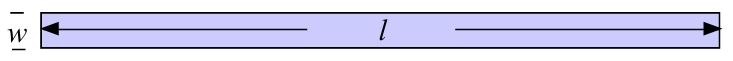
\includegraphics[width=.6\columnwidth]{imagenes/tirilla.jpeg}
		%\caption{Dibujo esquemático de un calibrador Vernier \cite{cita}.}
		%\label{fig:tirilla}
	\end{figure}

	El resultado del producto es $A=lw=15.59712\times 10^2 m^2$. Sin embargo, el número $15.59712\times 10^2$ tiene siete cifras significativas, mientras $w=4.62\times 10^{-5}m$ solo tiene tres cifras significativas. Por lo tanto, el resultado debe ser redondeado a tres cifras significativas: $A=15.6\times 10^2 m^2$ con una \textit{incertidumbre implícita} de $0.05\times 10^2 m^2$ de acuerdo a la \textit{regla 1}.\\

	En el caso de que se desee calcular la \textit{incertidumbre real} $\Delta A$ asociada al área, se debe tener en cuenta que la incertidumbre asociada a $l$ de $0.0005\times 10^7m$ y la de $w$ es $0.001\times 10^{-5}m$. Realizando el cálculo de la propagación (ver \cite{lanaturaleza}), se obtiene que $\Delta A= 0.019\times 10^2 m^2$, por lo que $A=(15.60 \pm 0.02)\times 10^2 m^2$. \\
	
	\textit{\textbf{Nota:}} Observe que para reportar la incertidumbre real esta tuvo que aproximarse a $0.02\times 10^2$ y al área tuvo que agregársele un decimal adicional $15.60\times 10^2$ que si bien cuenta como cifra significativa, no contradice la \textit{regla 2} pues solo se añade para dejar explicita la incertidumbre real en caso de que se solicite. \medskip 

	\section{Regla 3: Suma y Resta}

	La precisión de una suma o resta es igual a la del número menos preciso. \textit{\textbf{Ejemplo:}} considere la suma de $S = A + B = 3.37s + 0.042s$ con una incertidumbre de $\Delta A = 0.005s$ y $\Delta B = 0.0005s$. Con esta información, se tiene entonces que la suma $S$ no puede tener una precisión mejor que la de $A$, por lo que el resultado se reporta como $S = 3.41s$ con una incertidumbre de $\Delta S =0.005s$.  

	\section{Ejericicios}

	\begin{enumerate}
		\item Calcule el número correcto de cifras significativas: \textbf{(a)} $2.63g/4.982cm^3$, \textbf{(b)} $13.54millas/5.00h$ \textbf{(c)} $13.2g + 1.4688g + 0.04g$, \textbf{(d)} $(2g + 0.0127g + 459g)/(6.2cm^3-0.567cm^3)$.
		\item Exprese las siguientes cantidades en notación 	científica e indique el número de cifras significativas: \textbf{(a)} $0.0000034527$, \textbf{(b)} $335634$, \textbf{(c)} $3.1416$, \textbf{(d)} $0.096$.
		\item Redondee las siguientes cantidades hasta el numero indicado de cifras significativas (cs): \textbf{(a)} $132.505g$ (4cs), \textbf{(b)} $13.452lb$ (2cs), \textbf{(c)} $345onzas$ (2cs), \textbf{(d)} $7.4855g$ (3cs), \textbf{(e)} $11.698lb$ (1cs), \textbf{(f)} $12.05$ (3cs).
	\end{enumerate} 
	
	\printbibliography[heading=bibintoc]
	
\end{document}